\documentclass[a4paper,14pt]{extarticle}
\usepackage{../../tex-shared/report-layout}

\renewcommand{\mylabnumber}{2}
\renewcommand{\mylabtitle}{Сетевое и календарное планирование}
\renewcommand{\mysubject}{Управление IT-проектами}
\renewcommand{\mylecturer}{Смирнова Н.Б.}

\begin{document}
\begin{titlepage}
    
    \thispagestyle{empty}
    
    \begin{center}
        
        Министерство науки и Высшего образования Российской Федерации \\
        Севастопольский государственный университет \\
        Кафедра ИС
        
        \vfill

        Отчет \\
        по лабораторной работе №\mylabnumber \\
        \enquote{\mylabtitle} \\
        по дисциплине \\
        \enquote{\MakeTextUppercase{\mysubject}}

    \end{center}

    \vspace{1cm}

    \noindent\hspace{7.5cm} Выполнил студент группы ИС/б-17-2-о \\
    \null\hspace{7.5cm} Горбенко К. Н. \\
    \null\hspace{7.5cm} Проверил \\
    \null\hspace{7.5cm} \mylecturer

    \vfill

    \begin{center}
        Севастополь \\
        2020
    \end{center}

\end{titlepage}

\section{Цель работы}
Получение навыков составления сетевого и календарного плана работ, графиков
загрузки трудовых ресурсов, поиска перегруженности трудовых ресурсов.

\section{Задание на работу}
Составить календарный план для проекта:

Общая информация о проекте:
\begin{table}[H]
    \caption{Общая информация о проекте}
    \begin{tabular}{ | p{5.5cm} | p{11cm} | }
        \hline
        Наименование проекта & Разработка адаптивного сервиса для изучения иностранной лексики \\ \hline
        Краткое наименование проекта & Разработка адаптивного сервиса для изучения иностранной лексики \\ \hline
        Заказчик проекта & Севастопольский государственный университет \\ \hline
        Дата начала проекта & 01.03.2021 \\ \hline
        Дата окончания проекта & 31.06.2021 \\ \hline
    \end{tabular}
\end{table}

\section{Ход работы}
В результате анализа проекта выделим переччень работ по проекту и присвоим им
порядковые номера. Результаты размещены в таблице \ref{tab:tasks}.
\begin{table}[H]
    \caption{Перечень работ}
    \begin{tabular}{ | c | p{14.5cm} | }
        \hline
        № & \textbf{Название события} \\ \hline
        0 & Начало проекта \\ \hline
        1 & Утверждение и составление спецификаций, составление технического задания \\ \hline
        2 & Проектирование архитектуры системы \\ \hline
        3 & Выбор облачных поставщиков хостинга и баз данных \\ \hline
        4 & Выбор поставщиков внешних словарей \\ \hline
        5 & Разработка интерфейсов \\ \hline
        6 & Разработка программных модулей \\ \hline
        7 & Разработка пользовательского интерфейса \\ \hline
        8 & Интеграция интерфейса в программные модули \\ \hline
        9 & Разработка документации \\ \hline
        10 & Проведение тестирования \\ \hline
        11 & Конец проекта \\ \hline
    \end{tabular}
    \label{tab:tasks}
\end{table}

Установим для каждого события предшествующие события, до окончания которых оно
не может быть начато. Результат заносится в таблицу \ref{tab:prerequisites}.
\begin{table}[H]
    \caption{Перечень работ}
    \begin{tabular}{ | c | L{9.5cm} | L{5cm} | }
        \hline
        \textbf{№} & \textbf{Предшественники} & \textbf{Название события} \\ \hline
        0 & - & 0. Начало проекта \\ \hline
        1 & 0. Начало проекта & 1. Утверждение и составление спецификаций, составление технического задания \\ \hline
        2 & 1. Утверждение и составление спецификаций, составление технического задания & 2. Проектирование архитектуры системы \\ \hline
        3 & 1. Утверждение и составление спецификаций, составление технического задания & 7. Разработка пользовательского интерфейса \\ \hline
        4 & 2. Проектирование архитектуры системы & 5. Разработка интерфейсов \\ \hline
        5 & 2. Проектирование архитектуры системы & 3. Выбор облачных поставщиков хостинга и баз данных \\ \hline
        6 & 2. Проектирование архитектуры системы & 4. Выбор поставщиков внешних словарей \\ \hline
        7 & 2. Проектирование архитектуры системы \linebreak
            3. Выбор облачных поставщиков хостинга и баз данных \linebreak
            4. Выбор поставщиков внешних словарей \linebreak
            5. Разработка интерфейсов & 6. Разработка программных модулей \\ \hline
        8 & 6. Разработка программных модулей \linebreak
            7. Разработка пользовательского интерфейса & 8. Интеграция интерфейса в программные модули \\ \hline
        9 & 5. Разработка интерфейсов & 9. Разработка документации \\ \hline
        10 & 8. Интеграция интерфейса в программные модули & 10. Проведение тестирования \\ \hline
        11 & 9. Разработка документации \linebreak
             10. Проведение тестирования & 11. Конец проекта \\ \hline
    \end{tabular}
    \label{tab:prerequisites}
\end{table}

Для составления календарного плана нам понадобятся:
\begin{itemize}
    \item дата начала проекта;
    \item список участников проекта и их рапределение по работам.
\end{itemize}

В качестве даты начала проекта используем 01.03.2021 г. - понедельник.
Распределение исполнителей по работам приведено в таблице \ref{tab:executors}.

\begin{table}[H]
    \caption{Перечень работ}
    \begin{tabular}{ | c | L{9.5cm} | L{5cm} | }
        \hline
        0 & 0. Начало проекта & -- \\ \hline
        1 & Утверждение и составление спецификаций, составление технического задания & Менеджер проекта, архитектор \\ \hline
        2 & Проектирование архитектуры системы & Архитектор, бэкэнд разработчик, фронтенд разработчик \\ \hline
        3 & Выбор облачных поставщиков хостинга и баз данных & Архитектор, бэкэнд разработчик \\ \hline
        4 & Выбор поставщиков внешних словарей & Архитектор, бэкэнд разработчик \\ \hline
        5 & Разработка интерфейсов & Архитектор \\ \hline
        6 & Разработка программных модулей & Бэкэнд разработчик, фронтенд разработчик \\ \hline
        7 & Разработка пользовательского интерфейса & Фронтенд разработчик, дизайнер, UX дизайнер \\ \hline
        8 & Интеграция интерфейса в программные модули & Бэкэнд разработчик, фронтенд разработчик \\ \hline
        9 & Разработка документации & Бэкэнд разработчик, фронтенд разработчик \\ \hline
        10 & Проведение тестирования & Тестировщик \\ \hline
        11 & Конец проекта & -- \\ \hline
    \end{tabular}
    \label{tab:executors}
\end{table}

Далее следует составить календарный план проекта, который представлен в таблице
\ref{fig:calendar-plan}.

Каждая из работ таблицы \ref{tab:tasks} на сетевом графике обозначается дугой
длительностью. Вершины сетевого графа -- события плана. Результат изображен на
рисунке \ref{fig:net-graph}.
\begin{figure}[H]
    \centering
    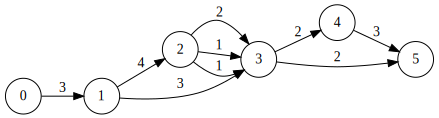
\includegraphics[width=\linewidth]{net-graph.gv.png}
    \caption{Сетевой график}
    \label{fig:net-graph}
\end{figure}

\begin{landscape}
\begin{figure}[H]
    \centering
    \includegraphics[width=\linewidth]{calendar-plan}
    \caption{Календарный план}
    \label{fig:calendar-plan}
\end{figure}
\end{landscape}

\section*{Выводы}
В ходе выполнения лабораторной работы были получены навыки составления сетевого
и календарного плана работ, графиков загрузки трудовых ресурсов, поиска
перегруженности трудовых ресурсов.
\end{document}